\section{Technical Considerations}

\subsection{Sentiment Analysis}

Once the user's online content has been extracted, it will then placed into one of the following categories: negative, positive or neutral. This can be achieved by performing sentiment analysis on the content. However, the app's back-end has to be first be trained by supplying sufficient training data.

The language used for the sentiment analysis will be Python. Moreover, the group will also make use of the Natural Language Toolkit (NLTK) Python library.

\subsubsection{Data Collection \& Pre-Processing}

The first step is to collect existing positive, negative and neutral content and store them in an array.

\begin{figure}
  \centering
  \begin{minipage}{14cm}
    \centering
    \inputminted[fontsize=\footnotesize]{python}{inc/snippets/collection.py}
    \caption{Content Collection}
    \label{fig:sentiment_analysis_step1a}
  \end{minipage}
\end{figure}

These words are then collected into a single list of tuples, each of which containing two elements.

\begin{figure}
  \centering
  \begin{minipage}{14cm}
    \centering
    \inputminted[fontsize=\footnotesize]{python}{inc/snippets/collection_iteration.py}
    \caption{Content Pre-Processing}
    \label{fig:sentiment_analysis_step1b}
  \end{minipage}
\end{figure}

\subsubsection{Classifier Creation}

Once sufficient content has been attained, a list of each word extracted from all the content needs to be collected and then ordered based on frequency of occurrence. This can be done by initially collecting all words and associating a frequency of occurrence to each and then ordering the list based on the frequency value. 

\begin{figure}
  \centering
  \begin{minipage}{14cm}
    \centering
    \inputminted[fontsize=\footnotesize]{python}{inc/snippets/classifier.py}
    \caption{Word Frequency}
    \label{fig:sentiment_analysis_step2a}
  \end{minipage}
\end{figure}

To create the classifier, relevant features needs to be captured via a feature extractor. Below shows the function implementation of this.

\begin{figure}
  \centering
  \begin{minipage}{14cm}
    \centering
    \inputminted[fontsize=\footnotesize]{python}{inc/snippets/classifierB.py}
    \caption{Feature Extraction}
    \label{fig:sentiment_analysis_step2b}
  \end{minipage}
\end{figure}

A training set will then be created using the NLTK library. Furthermore, a classifier object can be instantiated.

\begin{figure}
  \centering
  \begin{minipage}{14cm}
    \centering
    \inputminted[fontsize=\footnotesize]{python}{inc/snippets/classify.py}
    \caption{Classifier Training}
    \label{fig:sentiment_analysis_step2c}
  \end{minipage}
\end{figure}

\subsubsection{Classifier Testing}

\begin{figure}
  \centering
  \begin{minipage}[h!]{14cm}[h!]
    \centering
    \inputminted[fontsize=\footnotesize]{python}{inc/snippets/classifier.py}
    \caption{Classifier Training}
    \label{fig:sentiment_analysis_step3}
  \end{minipage}
\end{figure}

Now that the classifier has been created and trained, the sentiment analyser can be tested.

\begin{landscape}

\section{System Architecture Diagram}

\begin{figure}
  \centering
  \begin{minipage}{180mm}
    \centering
    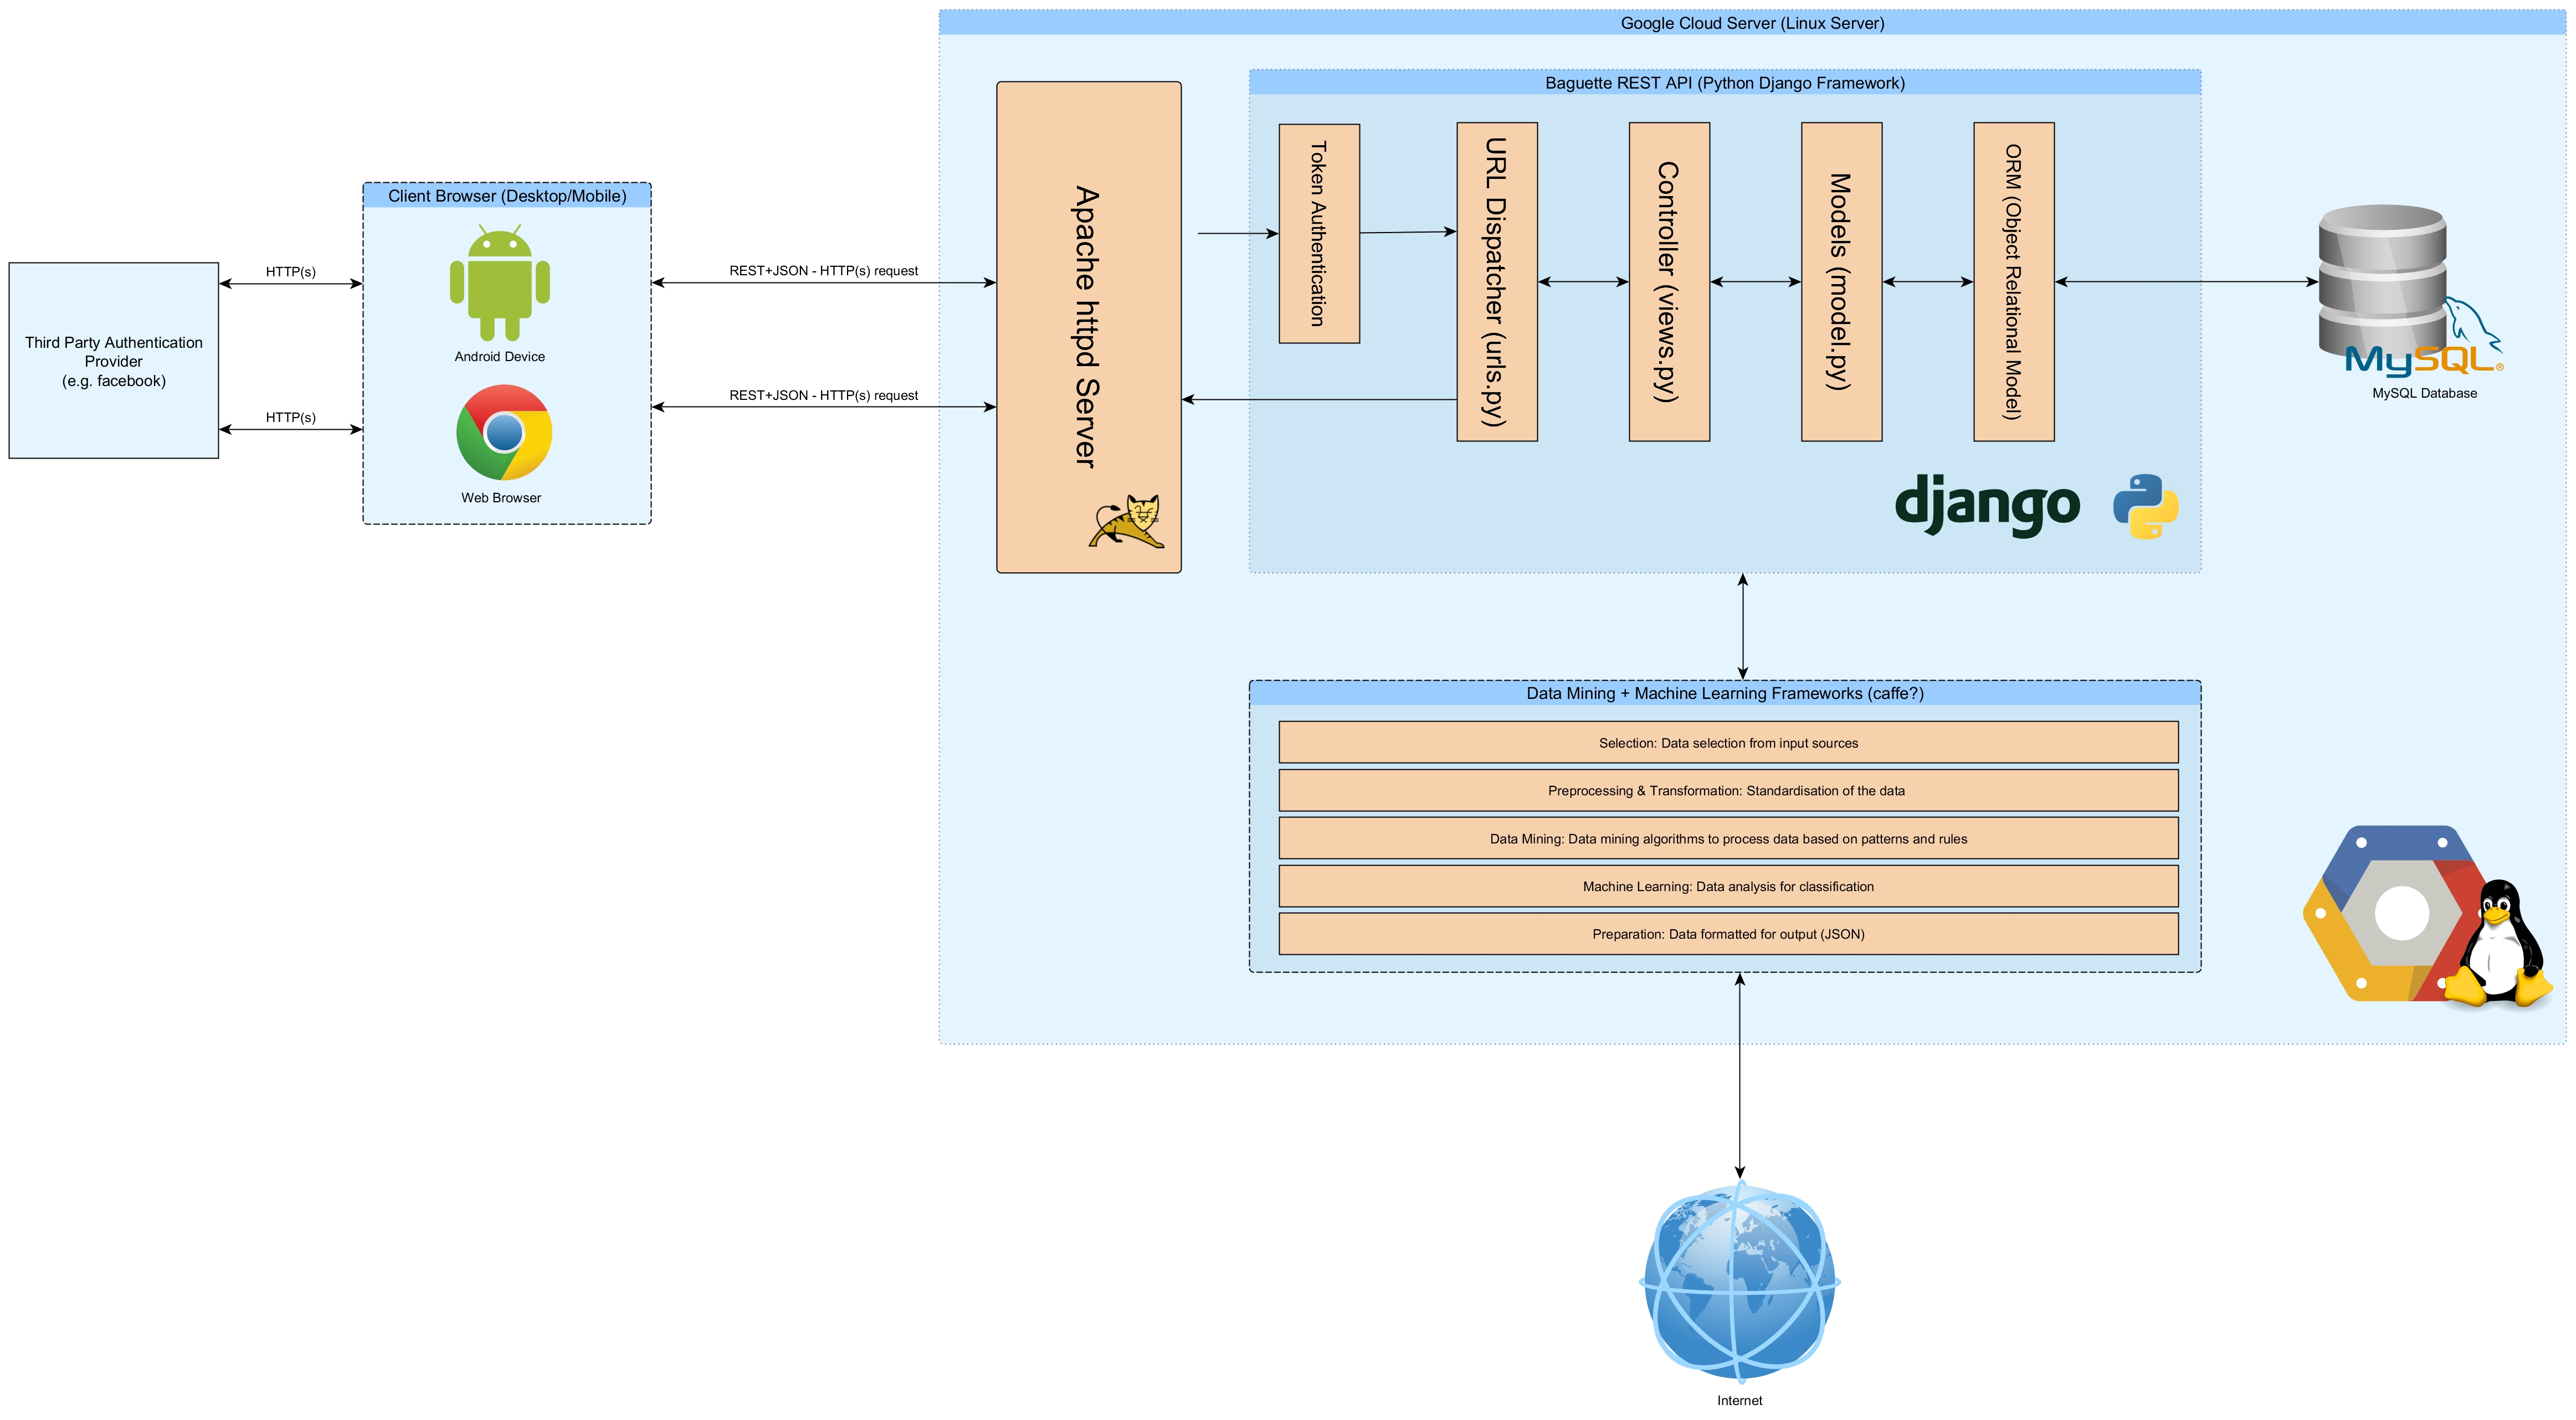
\includegraphics[width=180mm]{inc/architecture_diagram.jpg}
    \caption{System Architecture Diagram}
    \label{fig:architecture_diagram}
  \end{minipage}
\end{figure}

\end{landscape}
